\documentclass{beamer}
\usetheme{Warsaw}

\usepackage[utf8]{inputenc}
\usepackage{fancybox}
\usepackage{multimedia} 
\usepackage{subfig}
\usepackage{amsmath}
\usepackage{hyperref}
\usepackage[all]{xy}
\begin{document}


\title[Angewandte Mathematik] % (optional, only for long titles)
{Angewandte Mathematik
\\
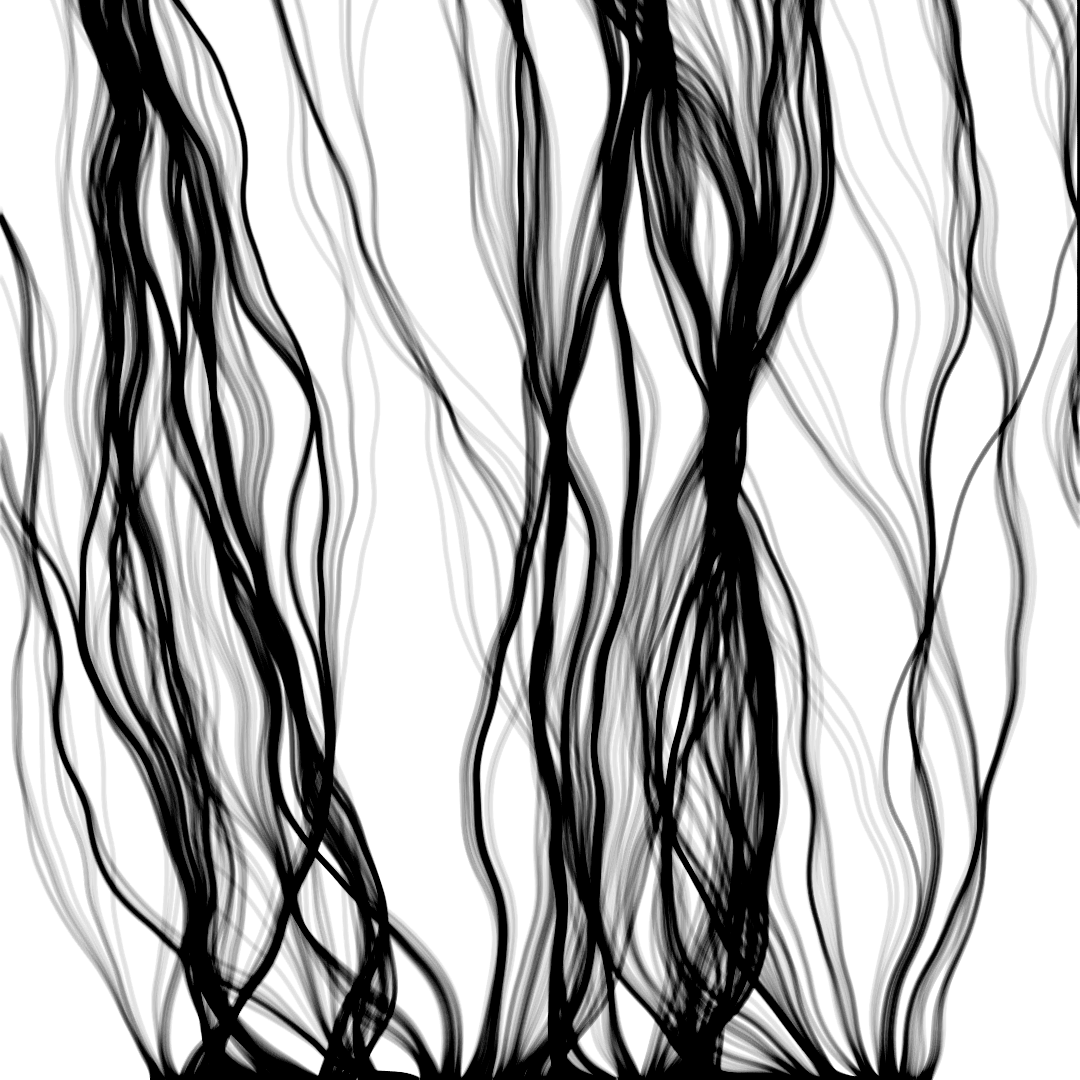
\includegraphics[scale=0.15]{images/cover}
}
\subtitle{}
\author[Dr. Johannes Riesterer] % (optional, for multiple authors)
{Dr.  rer. nat. Johannes Riesterer}

\date[KPT 2004] % (optional)
{}

\subject{Übungen zu Angewandte Mathematik}

\frame{\titlepage}




\begin{frame}
    \frametitle{Angewandte Mathematik}
\framesubtitle{Übung}
\begin{block}{Aufgabe 1}
Sei $f(x,y) := $. Berechnen Sie das Differential $df(1,1)$ so wie die Richtungsableitung $\partial_h f (1,1)$ für $h= $.
\end{block}
 \end{frame}


\begin{frame}
    \frametitle{Angewandte Mathematik}
\framesubtitle{Übung}
\begin{block}{Aufgabe 2}
Sei $c \in \mathbb{R}$ eine Konstante. Berechnen Sie für die  konstante Funktion $f(x) = c$ für alle $x \in \mathbb{R}^n$ die Richtungsableitung $\partial_h f(a)$.
\end{block}
 \end{frame}

\begin{frame}
    \frametitle{Angewandte Mathematik}
\begin{block}{Aufgabe 3}
Für das Differential einer differenzierbaren Funktion  $f: U \to \mathbb{R}$ gilt für alle $a \in U$:
\begin{itemize}
\item  $df(a) (h) :=  df(a) \cdot h$ ist eine lineare Abbildung von $\mathbb{R}^n$ nach $\mathbb{R}$.
\item $df(a)  \cdot h = \partial_h f(a)$. 
\item $d (f \cdot g) = g(a) d(f) + f(a) dg$
\item $d(f + g) = df + dg$
\end{itemize}
\end{block}
 \end{frame}


\begin{frame}
    \frametitle{Angewandte Mathematik}
\begin{block}{Aufgabe 4}
Sei $\gamma(t):= \begin{pmatrix} \cos(t) \\ \sin(t) \end{pmatrix}$ für $t \in [0, 2 \pi]$.
\end{block}
 \end{frame}



\end{document}

